\section{User Experience Strategy}
The app that this project is aiming at developing will have a focus on the intuitive user experience. To have a focus on intuitiveness means that we must be able to understand what that implies. The dictionary defines intuitive as: 
\begin{itemize}
\item perceiving directly by intuition without rational thought, as a person or the mind.
\end{itemize}
they define the concept of intuitiveness as human perception by intuition, what then is intuition? again the dictionary will provide a relatively easy answer: 
\begin{itemize}
\item intuition\\
\begin{enumerate}
\item The act or faculty of perceiving, or apprehending by means of the senses or of the mind; cognition; understanding.
\item immediate or intuitive recognition or appreciation, as of moral, psychological, or aesthetic qualities; insight; intuition; discernment:
an artist of rare perception.
\item the result or product of perceiving, as distinguished from the act of perceiving; percept.
\item Psychology. a single unified awareness derived from sensory processes while a stimulus is present.
\end{enumerate}
\end{itemize} from this definition it is clear that the concept of intuitiveness is a human concept, more specifically a human subconscious concept. In an article from 1994 Jef Raskin\cite{JRaskin} talks about how intuitiveness comes from familiarity, while the article is quite old the observations that he makes does support the idea that intuitiveness is directly linked with the targeted users. In the article Raskin talks about an experiment that he performed, where he asks a test participant to perform a certain task with a mouse, back in 1994 the mouse was still not a tool that was commonplace and as such the test subject had no familiarity with how to work with a mouse, and required help. Raskin showed the participant how to move the mouse in the correct manner, and instantly the participant knew how it worked and didnt require any more help, because as Raskin notes: \textit{"The directional mapping of the mouse was "intuitive" because in this regard it operated just like joysticks (to say nothing of pencils) with which she} [The test participant] \textit{was familiar"}\cite{JRaskin} this observation strongly supports the idea of intuition as familiarity. With this in mind the goal of this section becomes clear: first this section will first give brief overview of the topic of user experience. Next the section will try to define what the intuitive user experience is, and lastly how does the gained knowledge translate to being used as guidelines for making an intuitive mobile device app.  

\subsection{Introduction to user experience }\label{UXIntro}
A study of user experience\footnote{hereafter referred to as UX} is a study of how a user feels when interacting with a system. The field encompasses a whole range of different and seemingly unrelated topics. The most known part of UX is probably the concept of usability which will be discussed later in the section, other things make up UX, such as: Design, Accessibility, System performance, Ergonomics, human factors and more concepts\cite{UXIntro}. The term user experience  was originally coined by Dr. Donald Norman, who was the first to describe the importance of user-centered design. User-centered design is a design concept that lets the users dictate(to a certain degree) what the system should contain and what form it should take.
Before user-centered design the general design process looked like:
\begin{figure}[H]
\centering
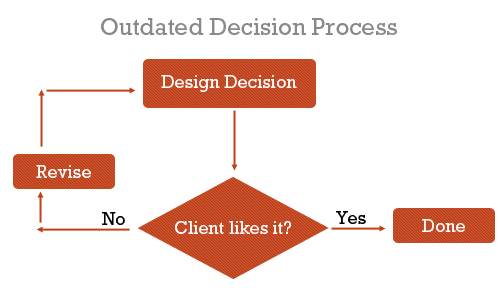
\includegraphics[scale=0.8]{OutDatedDecisionProcess.jpg}
\caption{old decision process, Jacob Gube 2010}
\end{figure}
nowhere in the design process was the users a factor, the design was simply made according to how the designers as well as the client felt it should be. making the same kind of chart for a user-centered approach would look:\\
\begin{figure}[H]
\centering
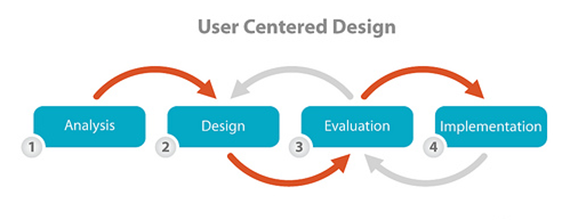
\includegraphics[scale=0.8]{UserCenteredDesign.png}
\caption{a chart of how user-centered design could function, Usabilla 2014}
\end{figure}
as this chart shows, user-centered design can be an iterative process. the grey arrow represents the user feedback, which shows that the users should be involved in the evaluation of a design.

User Experience and usability is often confused since a large portion of the guidelines for proper usability also applies to giving a good user experience. What sets the user experience apart from usability is that UX deals with the feeling of usage and usability deals with the effectiveness of usage
\todo{source for the example}An example of which could be the iBooks app for iPad.
\begin{figure}[H]
\centering
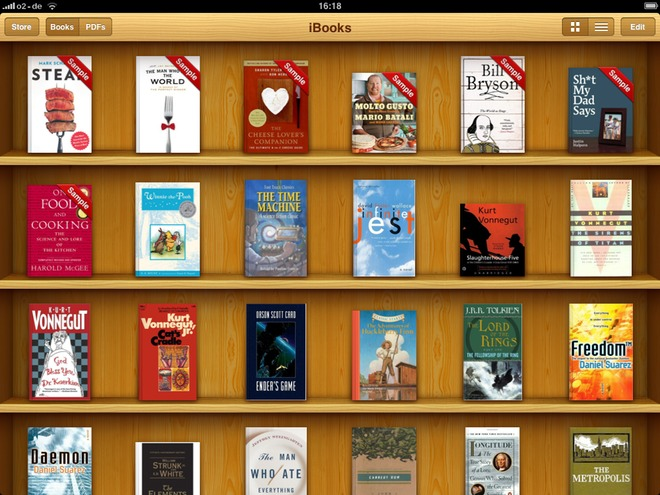
\includegraphics[scale=0.5]{iBooks.png}
\caption{Apple iBooks for comparison}
\end{figure}\todo{might need a source reference}

\begin{figure}[H]
\centering
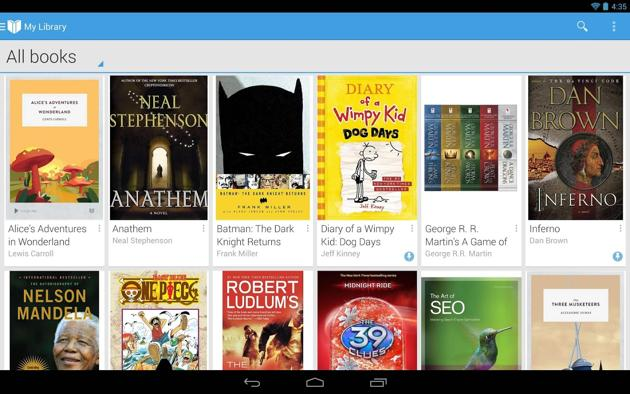
\includegraphics[scale=0.5]{GooglePlayBooks.png}
\caption{Google Play Books for comparison}
\end{figure}\todo{might need a source reference}
An application for reading and browsing E-books. The layout is simple, it provides an overview of the owned books with a visual representation of the covers which is common for such apps and as such, do not set itself apart from the state of the art when it comes to usability, however the user experience is greatly improved simply by changing the background to resemble a bookshelf, it makes the experience of logging onto IBooks resemble the experience of going into a book store or library a lot more, this approach relates to the concept of intuition as familiarity, which will be discussed in the next subsection.   



\subsection{Intuitiveness is familiarity}
as explained in the previous section \ref{UXIntro} user centered design is a main pillar of user experience, this is even more true when talking about intuition as a design concept. As Jared M. Spool mentions in his 2005 article \textit{People Intuit, not Interfaces}\cite{JaredMSpool} the article mentions that it is the users that define whether or not an interface is intuitive as the interface itself is nothing more than a collection of code. what this shows is that for an interface to be intuitive, a comprehensible knowledge about the targeted users' previous experience with similar interaction, is not only useful but absolutely crucial. the article introduces the concept of a knowledge space, which is the arbitrary space that holds all the knowledge that pertains to a given interface. 

\begin{figure}[H]
\centering
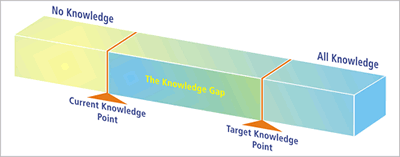
\includegraphics[scale=1]{KnowledgeSpace.png}
\caption{the knowledge space viewed as a continuous curve going from \textit{no knowledge} to \textit{all knowledge} \cite{JaredMSpool}}
\label{fig:Knowledge}
\end{figure}

as seen in figure: \ref{fig:Knowledge} there are two points of interest in the knowledge space that is the \textit{Current Knowledge Point} and the \textit{Target Knowledge Point} a brief explanation of the two points:
\begin{description}
 \item[\textbf{Current Knowledge Point}] \hfill\\
 This is the expected user knowledge which can be defined by a multitude of ways ie. user interviews, analysis of similar apps etc. figuring out what the current knowledge point is will enable the app to fill the knowledge gap without having to guide the user through every tiny detail. 
\item[\textbf{Target Knowledge Point}]\hfill\\
this is the amount of knowledge a user needs, to be able to use the app/programme as intended.
\item[\textbf{The Knowledge Gab}]\hfill\\
the knowledge gab is all the knowledge that the app/programme will have to provide to the user, this is usually done with a series of tutorials. 
\end{description}

He puts forth two conditions which he determines are the two conditions needed before users will classify an interface as being intuitive, these are:
\begin{itemize}
\item \textit{Both the current knowledge point and the target knowledge point are identical. When the user walks up to the design, they know everything they need to operate it and complete their objective.}
\item \textit{The current knowledge point and the target knowledge point are separate, but the user is completely unaware the design is helping them bridge the gap. The user is being trained, but in a way that seems natural.}
\end{itemize} 
of these two conditions the latter one will probably be of more use to the project as the navigation with the gyroscope will not be a control scheme that the user necessarily  have used before. Since the end product is going to introduce a uncommon way of interacting it will be important to know which kind of interaction will feel most intuitive for the user, that is where the iterative process will enable extensive testing of different interaction models, to determine the correct approach for our users.
\subsection{ Designing intuitively  }
The topics discussed the previous section help define what the app has to be able to do, but besides these ideas, besides these topics the project will look at the following two structures that can help create a pleasant UX:
\begin{itemize}
\item Clear Umbrella Structure\\
\textit{"The umbrella structure is the overall structure that lays out what the product can do for you"}\cite{UXKeys} the umbrella structure is a design pattern that helps the user immediately see what the interface can do. in a 2013 article Kyrie Robinson points to Apple's central phone app as a example of a prober implementation of this structure. Further she points out that the umbrella structure can easily become an obstacle if the interface has too many features within the umbrella. 
\item  Empowering Users to Complete Tasks Faster\\
 \textit{“When a user has a good experience, one of the first things they say that they liked about it is that it was fast. Since users “equate fast with easy,” }\cite{UXKeys} the app that this project will develop does not contain a wide range of features but is a relatively specialized app, while this diminishes the urgency of the app being fast, it should not be neglected. Robinson points to 6 ways of empowering the users effectiveness:
 \begin{enumerate}
 \item \textbf{Make the app work faster}\\
 this is a straight forward engineering problem, as better/less code results in a faster interface. 
 \item \textbf{Simplify your users’ work flow}\\
  this means cutting down on the amount of screens that the app employs.
 \item \textbf{Make sure your navigation is intuitive}\\\label{effectivenessP3}
 As talked about earlier intuition is related to familiarity and familiarity coupled with the umbrella structure mentioned above should be able to provide an intuitive navigation within the app.
 \item \textbf{Reduce the amount of text}\\
 in relation to the second point, if an app has a lot of text it will slow down the work flow of the user, at least in the beginning.
 \item \textbf{Examine your graphics}\\
 Robinson points to graphics as being an important part of how a user perceives an app, she urges to keep the graphics: \textit{"clean and not distracting"} 
 \item \textbf{Buttons}\\
 when making any kind of button make sure that the user never questions whether or not it is a button, further Robinson also encourages to give the buttons one word labels such as "send", "buy", "find" etc. of cause the words should represent the action that the button performs.
 \end{enumerate}\cite{UXKeys} 
\end{itemize} 
these points together with the intuitiveness discussion above should enable the app to provide a intuitive user experience. 

\subsection{Understanding our Users}\todo{Move this section}
Even though we have previously analysed out target group, when we want to focus on the user experience, further target group considerations has to be made, that is why this paper will next talk about the concept of understanding the users. Georgi Sardo provides three points that will help with the design process of the app:
\begin{itemize}
\item What are your users’ digital device skills? Are they used to working with digital devices and software applications?\cite{Sardo}
\item What are your users’ skills in using your application? Does the application revolve around their professional area?\cite{Sardo}
\item Is the application the focal point for your users? Or is their attention limited?\cite{Sardo}
\end{itemize}
these three points can help develop an app that will be focused on the users needs, which is at its core what UX is all about.